\section{Supplementary: Selected Related Research from Co-authors}
\label{sec:related}

It is impossible for a single paper to summarize all related research in this area. We refer to the other papers in this collection of papers published as part of this special issue. Therefore, we restrict our summary of related and selected research to activities conducted by the authors.

{\bf von Laszewski} has worked in the area of scientific workflows for about 30 years. This includes the introduction of a novel metacomputing framework \citep{las-99-loosely,las-94-ecwmf,las-96-ecwmf} that was used to schedule jobs in a distributed fashion on multiple supercomputers and also access supercomputers of significant architectural design. 
This was continued by the usage of workflows in problem-solving environments \citep{las-01-pse}. This was followed by integrating many of the conceptual designs into the Globus Toolkit with the first application using workflows as part of Grids \citep{las-00-sbc}. The lesson from this motivated us to focus on developing the Java Commodity Grid Kit (Java CoG Kit) \citep{las-06-workcoordination,
las-06-workflow-book,
las-06-exp-a,
las-05-workflowrepo,
las-05-workflow-jgc,
las-05-exp,
las-04-abstraction-j,
las-03-gridcomputing,
las-02-javacog,
las-00-grande,
las-01-cog-concurency}. 
During the peak of Grid Computing over 100 demonstrations on the Supercomputing exhibition floor used the Java CoG kit. As part of these activities, he pioneered a remote execution service InfoGramm 
\citep{las-02-infogram}
that in addition to serving as a service returning information about remote resources also allowed the execution of programs and scripts executed remotely as part of Grids allowing workflows to utilize multiple Grid resources at the same time. Early systems such as GridAnt \citep{las-04-gridant} 
did provide the ability to formulate Grid Workflows into frameworks familiar to Java developers. A much-enhanced workflow framework system was introduced into the  Java CoG Kit Karajan \citep{las-06-workflow-book} that in addition to using DAGs also allowed the specification of iterations into the workflow to help in the analysis of advanced photon source images and other applications. It also includes the introduction of futures \cite{friedman-futures}. Prior work to Karajan includes \citep{las-04-gridant,las-01-cog-concurency,las-96-ecwmf}. The availability of the loops allowed superior performance as the application-specific demands could be integrated. Workflows could be specified through an API, but also through the integration of XML specification. The workflows could be dynamic and changed based on runtime conditions. Some of the ideas from this work were continued into the Swift framework while leveraging the futures from Karajan in support of fast, reliable, loosely coupled parallel computation \citep{las--7-swift}. 
As part of the CoG Kit, von Laszewski and his colleagues also invented the first service controllable file transfer service with GUI to coordinate multiple file transfers. While this work was focused mostly on implementations done in Java, a new development using mostly Python was started with the Cyberaide toolkit \citep{las-09-ccgrid} that later on was renamed to Cloudmesh. As the name indicates the emphasis here was the integration of cloud resources rather than the focus of utilizing and enhancing the Globus Toolkit services. However, it also included initially the integration with Globus that focused on file transfer 
\citep{las-04-ftp-journal}
\citep{las-03-ftp}.
This tool could support many different cloud services from which some no longer exist such as Eucalyptus \cite{eucalyptus} and OpenCirrus \cite{opencirrus}. The services supported included execution services on AWS, Google, Azure, and OpenStack (KIT, and Chameleon Cloud). It also included data transfer services. The workflows emphasized here were not server-to-server services, but client-to-server services. One of the goals was to create workflows that let a scientific user develop workflows that can be controlled from their laptop in such a fashion that the workflows can be started and monitored from the laptop, allowing also the shutdown of the laptop and restart and discovering its state from ongoing workflow executions. 
The Cloudmesh toolkit \citep{las-17-cloudmesh} philosophy includes the distribution of a number of plugins into an extensible command line and command shell framework. While separating them into different packages extensions and different client needs can be fulfilled more easily because the user can select the needed plugins so that Cloudmesh offers a highly customizable solution for the different users. Early plugins include compute and file transfer resource services for AWS, Azure, Google, and OpenStack. However, most recently we have focused on experiment management which we describe in more detail within this paper due to the advent of large-scale HPC centers with the use of GPUs to increase computational capabilities. 
Additionally, von Laszewski participated in the efforts of Cylon for data engineering that simplifies data engineering workflow tasks \citep{cylon,cylon-radical}. 

Although we also worked on infrastructure provisioning for scientific
workflows that include image management
\citep{las-12-imagemanagement}, management of cloud infrastructures
including \citep{las-20-10gce,las-14-bigdata,las-12-fg-bookchapter}
\citep{las-17-futuregrid} and creation of virtual clusters
\citep{las-16-virtcluster,las-19-harc-comet}, as well as federation
\citep{las-08-federated-cloud}, we will not discuss them here in more
detail and refer to the provided references as they also provide
valuable lessons in regard to integration of provisioning into
workflows.


\begin{figure}[p!]
  \centering
  \resizebox{12.5cm}{!}{%
\begin{forest}
skan tree
   [Supporting Workflow Concepts
        [Abstraction \citep{cloudmesh-ee}
          [YAML \citep{cloudmesh-ee}
            [DAG \citep{cloudmesh-ee}]
            [Array \citep{cloudmesh-ee}
              [Loop \citep{cloudmesh-ee}] 
            ]
          ]
          [Loop \citep{cloudmesh-ee}]
          [DAG \citep{cloudmesh-ee}]
        ]
        [Programming
           [GUI \citep{cloudmesh-cc,las-03-ftp,las-05-workflow-jgc}]
           [Portal \citep{las-99-rostock,las-06-guss-j,las-01-pse,las-02-cactus-j}]
           [Shell \citep{cloudmesh-ee}
             [Command line \citep{cloudmesh-ee}]
             [Command Shell \citep{cloudmesh-ee}]
             [Tools
                [Makefile]
                [Ant \citep{las-04-gridant}]
                [ ... ]
             ]
           ]
           [Scripting \citep{cloudmesh-ee}
              [Templating]
           ]
           [API \citep{las-02-javacog,las-17-cloudmesh}
             [Python \citep{cloudmesh-ee}
             [Loop \citep{cloudmesh-ee}]
             [DAG \citep{cloudmesh-ee}]
             [Array \citep{cloudmesh-ee}]
             [AI External Workflow Coordination Frameworks]
             ]
           ]
           [Dataframe \citep{cylon,cylon-radical}]
        ]
        [Runtime Support
           [Automation]
           [Monitoring \citep{cloudmesh-ee}
              [XDMoD]
           ]
           [Instrumentation \citep{cloudmesh-stopwatch,cloudmesh-gpu}]
           [Checkpointing \citep{las-2023-mlcommons-edu-eq}]
           [Benchmarking \citep{cloudmesh-ee}]
           [Reproducibility \citep{cloudmesh-ee}
               [cloudmesh FAIR suppport\citep{cloudmesh-ee}]
           ]
        ]
        [Resource Management
          [Remote Access \citep{cloudmesh-vpn}]
          [Federation \cite{las-08-federated-cloud,las-12-fedcloud-proc,antypas2021}]
          [Provisioning \citep{las-19-harc-comet,las-17-comet}]
          [Image Management \citep{las-12-imagemanagement}]
          [Scheduling
            [Cost \citep{las-01-greed}]
            [Energy ]
          ]
        ]
        [Standardization 
          [NIST]
        ]
        [Applications
            [AI
               [MLCommons]
               [Surrogates \cite{brewer2021production}]
            ] 
        ]
        [Evaluation 
           [Bibliography]
        ]
   ]
]
\end{forest}
}
   \caption{Scheduling challenges applied to all levels. We added not
     all but selected publications that we worked on as part of these
     workflow challenges.} 
  \label{F:graph-challanges}
\end{figure}



{\bf Brewer} has most recently focused on  {\bf Surrogate Model Workflows}. Figure \ref{fig:surrogate} provides a schematic of a typical machine-learned \textit{surrogate model} training and deployment workflow. Simulations are run on HPC using a variety of input parameters, from which data is extracted to curate a training dataset. Intelligent subsampling techniques, such as the principal of maximum entropy \cite{brewer2023entropy}, are used to curate an optimal training dataset. Hyperparameter optimization, such as DeepHyper \cite{balaprakash2018deephyper} or DLEO \cite{martinez2018deep}, is used to perform neural architecture search (NAS) in order to design an optimal architecture. Model validation techniques, such as using PI3NN \cite{liu2021pi3nn} use prediction intervals to assess proper coverage of the training data (in-distribution vs. out-of-distribution) via uncertainty quantification. Finally, optimal deployment studies are performed to determine the optimal deployment parameters, such as concurrency, batch size, and precision \cite{brewer2021production}. The surrogate model may be deployed as a means of replacing a computationally expensive portion of the simulation, for example, the machine-learned turbulence model \cite{bhushan2021development}, or replace the entire simulation, e.g., FourCastNet climate model \cite{pathak2022fourcastnet}.

A digital twin is a virtual replica of a physical asset, that mimics the behavior of the asset, and communicates in a bi-directional manner with its physical counterpart \cite{nas2023foundational}.   Brewer et al. \cite{brewer2024digital} recently developed a digital twin framework for HPC, called ExaDigiT, which integrates five different levels of information: (1) 3D asset modeling and visualization using augmented reality (AR), (2) telemetry/sensor data streaming from the physical asset, (3) machine learned (ML) models to mimic behavior in a data-driven manner, (4) modeling and simulation to mimic behavior based on first principles, and (5) reinforcement learning. Telemetry data is used for training AI/ML models and validating modeling and simulation. Modeling and simulation are used as a training environment for training a reinforcement learning agent, which provides autonomous control and optimization in the form of a feedback agent to the physical asset. This framework has been used to develop a digital twin of the Frontier supercomputer, the first Exascale supercomputer, which can dynamically schedule system workloads, predicts power at any level of granularity (from chip-level to total system) and cooling throughout the system and its supporting central energy plant, as well as dynamically predicts its power usage effectiveness (PUE). Such a twin can be used for performing what-if scenarios (e.g., what-if a pump fails), system optimizations (e.g., power and cooling), and virtual prototyping of future systems. Several different instantiations of data center digital twins are reviewed in \cite{athavale2024digital}. A benchmark has yet to be developed for such a complex workflow, but we plan to work on this in the future. 


\begin{figure}
    \centering
    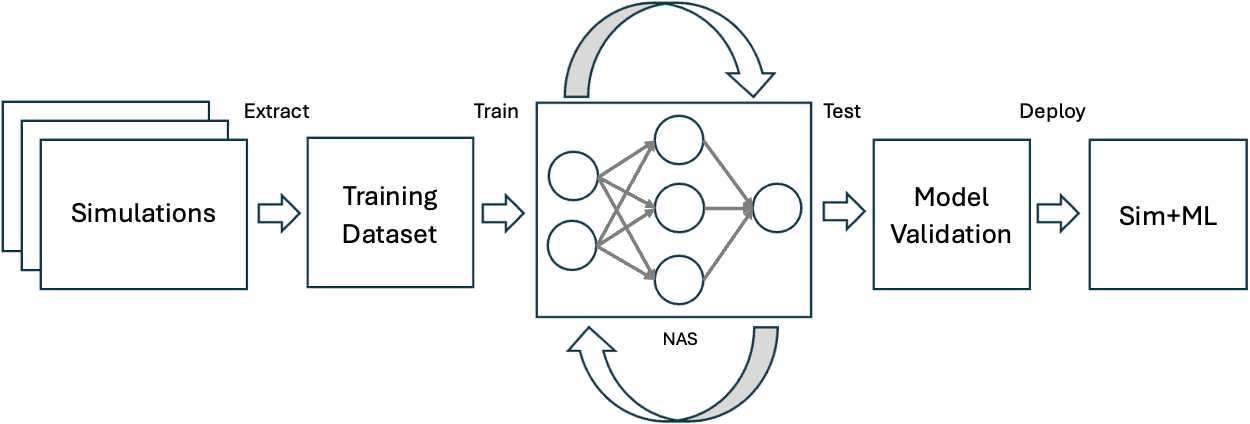
\includegraphics[width=0.8\linewidth]{images/workflow-surrogate-model.png}
    \caption{Machine-learned surrogate model training and deployment workflow \cite{brewer2023entropy}.}
    \label{fig:surrogate}
\end{figure}

\begin{figure}
    \centering
    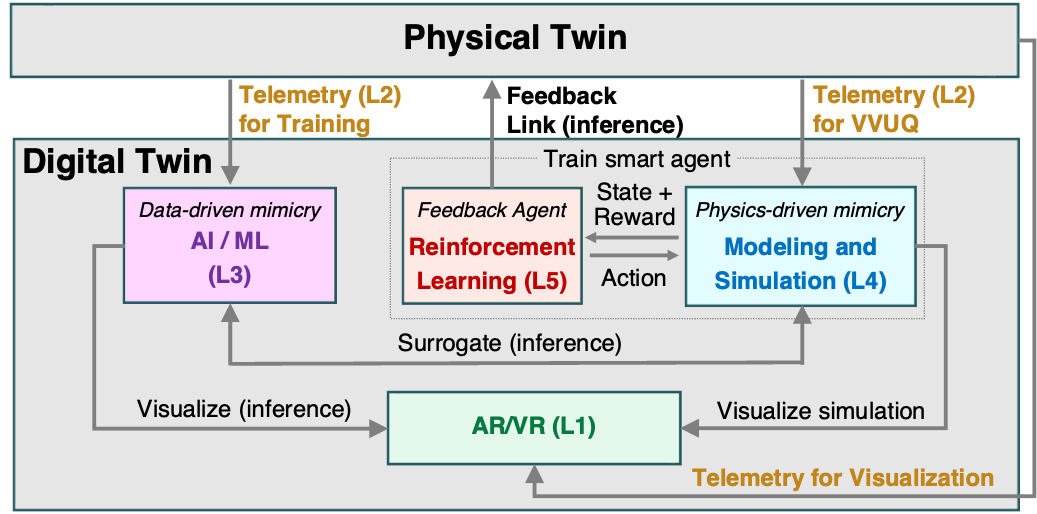
\includegraphics[width=0.8\linewidth]{images/workflow-digital-twin.png}
    \caption{Digital twin workflow \cite{brewer2024digital}.}
    \label{fig:dt}
\end{figure}

{\bf Wilkinson} has published recently on numerous topics in the area of scientific workflows \citep{ferreira_da_silva2024, ferreira_da_silva2022, badia2024integrating}, including work that incorporates benchmarks \citep{coleman2022-2}, cross-facility resources \citep{antypas2021}, provenance \citep{souza2023}, HPC \citep{wilkinson2022-2}, and quantum computing \citep{bieberich2023} for domains such as high-energy physics \citep{ananthraj2018}, bioinformatics \citep{lee2021,wilson2021}, and geology \citep{mcclure2020}. The main focus of his current work is on the application of the FAIR principles to computational ecosystems generally and computational workflows specifically \citep{wilkinson2022, caw2021-report}, the latter for which he co-chairs the Workflows Community Initiative's FAIR Computational Workflows working group, which recently published the results from its first two years \citep{wilkinson2025}. He also contributes to and co-administers WorkflowHub \citep{gustafsson2024}, and he serves in the GO FAIR US Office.

{\bf Shao} approaches workflow management from both the point of view of a domain scientist (with a particular emphasis on climate modeling) and a computer scientist investigating the emerging workflow paradigms and philosophies needed to combine AI/ML techniques with HPC-scale scientific simulations. In particular, most traditional numerical modeling operates as a pipeline with each stage focusing on the execution of a single application and the file system used to exchange data between stages. Ensemble-based modeling (often used in climate/weather) represents a horizontally scaled pipeline. Each individual member ensemble may differ by the values of their tunable parameters and/or the initial/boundary conditions, but run independently of each other. HPC simulation and AI applications often require a more asynchronous computational paradigm with data exchange that occurs across loosely coupled components (i.e. processing elements transfer data through an intermediary). The SmartSim library provides well-maintained, open-source tooling that enables domain scientists to describe and execute their own complex workflows.

While originally designed for in-the-loop inference, increasingly the library has been used by users whose workflows apply AI techniques to ensembles of simulation including reinforcement learning. In general, these are characterized by a more complex set of outcomes/artifacts than traditional scientific modeling. Instead of just simulation data, workflow artifacts may include trained AI models or control schemes to be used in conjunction with digital/physical twins. 

{\bf Kirkpatrick} collaborates with workflow experts at several NSF and DOE-funded labs. Activities have included an invited keynote at a recent international workflows workshop, activities through GO FAIR US to promote the extension of the FAIR Principles for Workflows, and participation in other workshops \cite{kirkpatrick2023}. Her most recent scholarship includes a co-authored a section from a Dagstuhl seminar proceeding, ``Integrating HPC, AI, and Workflows for Scientific Data Analysis'' on sustainability in HPC and AI-driven scientific workflows \citep{badia2024integrating}.

{\bf Pitkar} has more than 20 years of experience in the field of Information Technology. He is currently working as an IT Engineering Leader at Cummins Inc. in the Engineering and Automation department. He is passionate about automation and leads the Kubernetes platform team. His areas of focus are Platform Engineering, Cloud computing and automation.


{\bf Fleischer} works with open-source computer-vision applications towards traffic management and pedestrian safety analysis. The completion of an accurate object-detection model requires an integrated workflow process, from data annotation to configuring learning parameters using the Darknet/YOLO (You Only Look Once) suite~\citep{charette_2022, bochkovskiy2020yolov4optimalspeedaccuracy}. As standardized benchmarking is only feasible within containerized environments, he uses platforms such as Docker and Apptainer to facilitate portable training in HPC environments. Under the supervision of von Laszewski, he has conducted similar model training experiments on applications such as earthquake and meteorological forecasting.



To provide a better view of the various aspects of workflows we have organized them into a graph as shown in Figure \ref{F:graph-challanges}.


%\section{Workflow Use case for EKS Cluster in Amazon}
%Harshad writes after README.md completed



% \bibliographystyle{Frontiers-Harvard}
\newpage

\bibliographystyle{Frontiers-Vancouver} % Many Frontiers journals
% use the numbered referencing system, to find the style and resources
% for the journal you are submitting to:
% https://zendesk.frontiersin.org/hc/en-us/articles/360017860337-Frontiers-Reference-Styles-by-Journal

\bibliography{%
vonLaszewski-frontiers-citations}

\end{document}


\begin{comment}
\TODO{ move Authentication and Authorization, to the cloudmesh section

To simplify access to several resources, we have developed additional libraries within Cloudmesh, supporting newer technologies going beyond the use of SSH. This includes the introduction of a split-VPN library and toolkit that allows accessing multiple VPNs dependent on which resource is being used and through which VPN this resource is being secured. However problems still can arise if an organization decides not to deploy the capability of supporting split-VPN. We believe properly deployed VPN with the capability of split-VPN promotes the integration of heterogeneous distributed HPC resources which otherwise is not easily possible. This approach has the advantage that no additional services need to be deployed on the resources as they are already typically deployed.

Alternatively, the Superfacility API \citep{Enders2020} proposes an externally accessible API (with authentication) that allows users to perform basic workflow tasks. With the correct requests, users can interact with the workload manager, upload/download files, and run shell commands. The primary downside to this approach is that it requires owners of the HPC platform to deploy and support this API.
}
\end{comment}
